\documentclass[a4paper,12pt]{article}
\usepackage[ngerman]{babel}
\usepackage{multirow}
\usepackage{xltxtra}
\usepackage[utf8x]{inputenc}
\usepackage{fontspec}
\usepackage{eurosym}
\usepackage{graphicx}
\usepackage[paper=a4paper,left=25mm,right=25mm,top=25mm,bottom=25mm]{geometry}
\usepackage{makecell}
\usepackage[table]{xcolor}
\usepackage{float}
\usepackage[normalem]{ulem}
\usepackage{xcolor,colortbl}
\definecolor{Gray}{gray}{0.85}
\usepackage[automark]{scrlayer-scrpage}
\usepackage[
	colorlinks=true,
	urlcolor=blue,
	linkcolor=green
]{hyperref}
\setlength{\parindent}{0em}
\setlength{\parskip}{1ex}
\pagestyle{scrheadings}
\clearscrheadfoot
\usepackage[defaultsans]{droidsans}
\renewcommand*\familydefault{\sfdefault}
\begin{document}
\input{theme.tex}
\input{version.tex}
\ohead{Regelstand: \commitDate, id: \commitID}
\title{\tagYear\ SUMO Challenge Regeln}

\makeatletter
\let\inserttitle\@title
\makeatother
\begin{center}
	\rrgerLogo
	\huge                      % Schriftgröße einstellen
	\bfseries                   % Fettdruck einschalten
	\\
	\inserttitle
\end{center}

\section{Ziel}
Entwurf, Bau und Programmierung eines autonomen Roboters, der einen
gegnerischen Sumoroboter suchen und aus einem erhöhten Ring schieben kann.

\section{Divisionen/Massenklassen}
Bitte entnehmen Sie der untenstehenden Tabelle, in welcher
Division/Massenklasse Sie teilnehmen möchten.
\begin{center}
	\begin{tabular}{|c|c|c|} \hline
		\multirow{2}*{1kg} & \multirow{2}*{2kg} & Nur LEGO 1Kg \\
		& & (Optional) \\ \hline
		ES &  & ES \\ \hline
		MS & ** & MS \\ \hline
		HS & HS & HS \\ \hline
		** & UP & ** \\ \hline
	\end{tabular} \\ \vspace{\baselineskip}
\end{center}

\section{Roboter}
Autonomer Roboter, jede beliebige Plattform, der 1.500 USD oder weniger kostet
und die folgenden Designbeschränkungen erfüllt, die beim Robot Check-In
überprüft werden.
\begin{itemize}
	\item Die maximale Größe des Roboters beträgt 25 cm x 18 cm ohne
		Höhenbeschränkung, gemessen mit allen beweglichen Komponenten
		in ihrer Ausgangsposition.
	\item Größen- und Massenbeschränkungen werden während der gesamten
		Veranstaltung strikt durchgesetzt, um den Wettbewerb für alle
		Teilnehmer fair zu gestalten.
	\item Gelenkige oder bewegliche Komponenten sind zulässig, solange sie
		den oben genannten Konstruktionsregeln entsprechen. Es gilt
		jedoch die Regel "`kein vorsätzlicher Schaden"' - das bedeutet,
		dass Flossen und Gleitplatten zwar in Ordnung sind, aber
		absichtlich zerstörende Mechanismen wie Schleifspinner oder
		Hämmer etc. nicht erlaubt sind.
	\item In der Division "`Nur LEGO 1Kg"': Jeder LEGO-Roboter kann
		verwendet werden, muss aber vollständig aus LEGO-Markenteilen
		bestehen, autonom sein und den Designvorgaben entsprechen.
\end{itemize}

\section{Wettbewerbsring}
Ein schwarzer Kreis mit 100 cm Durchmesser und 5 cm weißem Rand auf 13 bis 20
mm dicker Platte. Die Oberfläche des Rings sollte 50 bis 80 mm über dem Boden
liegen. (die Maße werden je nach den verwendeten lokalen Materialien leicht
variieren).

\includegraphics[width=1.0\textwidth]{images/sumo_bot_ring.png}

\section{Allgemeine Spielregeln und Punktevergabe}
\begin{itemize}
	\item Jeder Roboter wird in einer Reihe von Wettkämpfen nach der
		"`Reihum-Methode"' antreten. Die Anzahl der Runden/Matches
		werden am Tag des Wettkampfes auf der Grundlage der Zeit und
		Anzahl der Roboter in jeder Kategorie bestimmt.
	\item Ein Spiel ist beendet, wenn eine Mannschaft zweimal gegen ihren
		Gegner gewonnen hat. 3 Punkte die für einen Sieg, 1 Punkt für
		ein Unentschieden und 0 Punkte für eine Niederlage vergeben
		werden.
	\item Die Punkte der Mannschaften werden während des Wettkampfs
		ausgezählt und angezeigt. Die besten 8 Mannschaften in jeder
		Kategorie werden für die Endspiele ausgewählt.
	\item Die Mannschaften können auf offenen Spielfeldern trainieren,
		wobei sie sich mit anderen trainierenden Teams abwechseln
		müssen.
	\item Die Roboter beginnen, indem sie die weiße Linie an den einander
		gegenüberliegenden Seiten des Tisches berühren. Sie können in
		jeder beliebigen Ausrichtung positioniert werden. Die Roboter
		müssen nach dem Drücken der Starttasten 3 Sekunden lang
		pausieren, damit das Teammitglied sich vom Ring zurückziehen
		kann.
	\item Der Verlierer ist der Roboter, der den Ring zuerst verlässt, was
		als Berührung der Oberfläche definiert ist, auf der der
		Wettbewerbsring platziert ist. Der Schiedsrichter kann nach 60
		Sekunden ein Unentschieden ausrufen oder bei "`gesperrten
		Robotern"' nach 5 Sekunden einen Neustart erzwingen, wenn er
		dies für richtig hält.
	\item Die Roboterbediener dürfen ihre Roboter nicht berühren, es sei
		denn, der Schiedsrichter weist sie dazu an. Pro Spiel werden 5
		Minuten zugeteilt, wenn es in dieser Zeit keinen Sieger gibt,
		wird es als unentschieden gewertet.
	\item Konfliktlösung - während des Spiels sind die Entscheidungen des
		Schiedsrichters endgültig.
\end{itemize}


\section{Turnierplan}
\begin{itemize}
	\item Wir veranstalten in der Regel Turniere für die besten 8
		Mannschaften. Sollte es jedoch aufgrund von Gleichstand mehr
		als 8 Teams geben, kann der Veranstaltungsleiter die
		Turniergröße auf 12 oder 16 erhöhen oder ein Turnier mit
		Gleichstand veranstalten, um auf 8, 12 oder 16 Teams zu kommen,
		die ein Turnier ausrichten.
	\item Die aufsteigenden Teams werden entsprechend ihrer Gesamtpunktzahl
		in die Turnierklasse gesetzt. Unten sehen Sie ein Beispiel für
		unsere typische 8-Mannschafts-Turnierrunde.
	\item Der zweite Platz ("`Runner Up"') wird verwendet, um den 3. Platz
		auf der Grundlage des Ergebnisses der Halbfinalrunde zu
		bestimmen.
\end{itemize}
\begin{figure}[H]
	\centering
	\def\svgwidth{\columnwidth}
	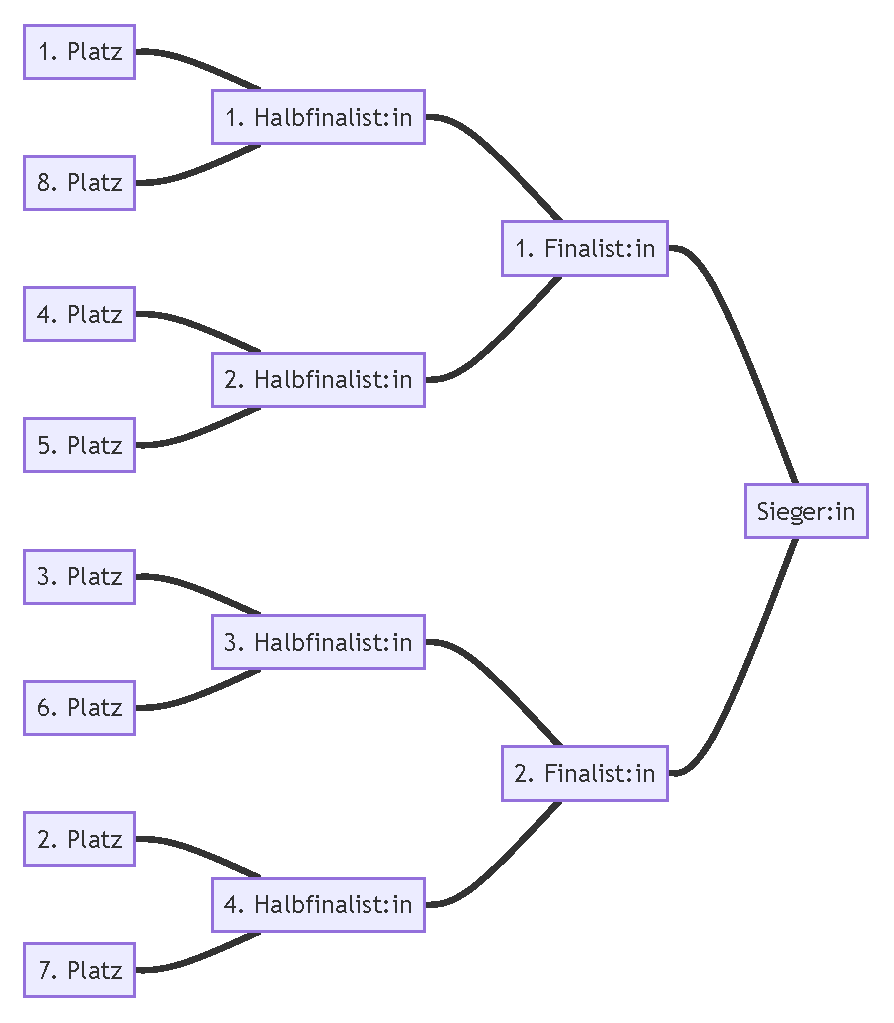
\includegraphics{tournament_score/tournament_score.pdf}
\end{figure}
\end{document}
